% LaTeX resume using res.cls
%
% Millar Resume, \LaTex style
%


\documentclass[margin]{res}
%\usepackage{helvetica} % uses helvetica postscript font (download helvetica.sty)
%\usepackage{newcent}   % uses new century schoolbook postscript font 
\usepackage[pdftex]{graphicx}
\setlength{\textwidth}{5.1in} % set width of text portion

\begin{document}

% Center the name over the entire width of resume:
 \moveleft.5\hoffset\centerline{\large\bf David W Millar}
% Draw a horizontal line the whole width of resume:
 \moveleft\hoffset\vbox{\hrule width\resumewidth height 1pt}\smallskip
% address begins here
% Again, the address lines must be centered over entire width of resume:
 \moveleft.5\hoffset\centerline{140 Levering Street}
 \moveleft.5\hoffset\centerline{Philadelphia, PA 19127}
 \moveleft.5\hoffset\centerline{david.w.millar@gmail.com}
 \moveleft.5\hoffset\centerline{http://resume.github.com/?david-w-millar}
 \moveleft.5\hoffset\centerline{610.304.8828}


\begin{resume}

\section{Summary}
  Seasoned software engineer with insatiable technolust.  Eager to crush complexity with elegant design.
  Well versed in OOA/D, web application architecture and infrastructure, security, the java ecosystem, networks, and messaging systems.
	Experience supporting the full systems development life-cycle and integration of production enterprise applications, public multitenant web applications, and research oriented projects.
  Invested in agile practices, contiunous process improvement, automation, and DevOps.
\section{Experience}

  {\sl Senior Software Engineer} \hfill	March 2012  -- July 2012 \\
  {\sl Software Engineer Contractor} \hfill	Dec 2011 -- March 2012 \\
  MDconnectME Inc \\
  Philadelphia , PA
  \begin{itemize} \itemsep -2pt %reduce space between items
    \item Worked in a senior capacity on planning, design, requirements, developing and maintaining infrastructure for the MDconnectME application: a public web-facing JEE/Spring/Hibernate/Jsp/jQuery based application.
    \item Many hats were worn: data architecture, persistence, security, UX, etc.  Major focus on simplicity, scalability, cross-browser support, and HIPAA compliance.
    \item Designed, developed, and maintained back-end messaging systems and infrastructure using Amazon EC2 for SMS and e-mail.
  \end{itemize}


  {\sl Software Engineer} \hfill	June 2011 -- March 2012 \\
    Yellowbook Inc \\
    King of Prussia, PA
    \begin{itemize} \itemsep -2pt %reduce space between items
      \item Developed and maintained software systems to manage Yellowbook's repository of digital business listings, advertisements, and related artifacts along with a web application for data management.
            Interfaced with several other systems including the CDN, artwork workflow, search, web, in-house ratings and review system, and billing.
      %\item Developed and maintained software to provide listing feeds to 3rd parties (including Google, Citygrid, and TomTom)
      \item Ported some ETL applications from C\# to Java, managed an off-shore development team of three, and decreased chaos by leveraging PM tools.
      \item Experimented with Behavior-Driven Development in order to allow business analysts to write unit tests in plain english.
    \end{itemize}


  {\sl Research Engineer} \hfill	November 2008 -- April 2011 \\
    Drexel University ACIN Center \\
    Camden, NJ 
    \begin{itemize}  \itemsep -2pt %reduce space between items
      \item Managed and oversaw the completion of several projects under contract with the DoD and assisted in writing proposals to acquire multi-million dollar contracts.
      \item Researched, developed, and analyzed reliable group messaging systems on resource constrained networks using wireless network emulation.
            Won a research award from the Naval Research Labs for a paper that analyzed the performance of one system, which is now on the fast track to deployment in the field.
      \item Participated in live Command, Control, Communications, Computers, Intelligence, Surveillance and Reconnaissance (C\textsuperscript{4}ISR) exercises  with domestic forces. Supported coalition experiments with the German and French.
      % \item Designed network-centric middleware for a C\textsuperscript{2} system based on SOA and intelligent agents, along with biometric profile dissemination software
    \end{itemize}

  {\sl Software Engineer} \hfill	September 2003 -- November 2008 \\
    Resource Utilization and Management Group \\
    Comcast, Mount Laurel, NJ
    \begin{itemize}  \itemsep -2pt %reduce space between items
      \item Worked closely with consultants to develop and optimize an IP Address Management system supporting over 2,000 users and hosting information for Comcast's national infrastructure and millions of customers.
      \item Supported the full systems life-cycle of SOA based solutions to automate workflows and integrate enterprise systems and business processes.
            These included IP Address management, IP provisioning, user workflows, and asset management.
            This allowed for Comcast's footprint to grow with minimal user intervention, and saved several man-days of work daily.
      % \item Optimized IP address management system for high availability and redundancy
      % \item Developed software to mass import customer information from acquisitions
     \end{itemize} 

%Sungard Computer Recovery Services, Philadelphia, PA
% LAN Recovery Specialist for midrange workgroups, Summer of 2000
% Assisted in the configuration of NT servers
% Organized scheduling for clients

\section{Education} {\sl Bachelor of Science,} Computer Science \\
   % \sl will be bold italic in New Century Schoolbook (or
   % any postscript font) and just slanted in
   % Computer Modern (default) font
   Drexel University, Philadelphia, PA \\
   Concentrations: Data Structures and Algorithms and Operating Systems


% This needs some serious work
% TODO: Figure out a way to better organize this %
\section{Computer \\ Skills}
\begin{list}{}%
{\leftmargin=1em \itemindent=-1em}
  \item \textbf{\textit{Operating Systems:}} Linux, OS X, Windows, Various Unix, Android
  \item \textbf{\textit{Languages:}} Java, Groovy, SQL dialects, \LaTeX, various scripting, markup, and templating. Capable of learning new languages.
  \item \textbf{\textit{CASE Tools: }} Eclipse, Intellij IDEA, gradle, maven, ant, svn, mercurial, jenkins/hudson, artifactory, redmine
  % \item \textbf{\textit{Databases: }} SQL Server, mysql, PostgreSQL
  \item \textbf{\textit{Frameworks: }} Spring, Hibernate, Grails, angularjs, jQuery, various web, testing, and AJAX frameworks
  \item \textbf{\textit{Other: }} vim, apache httpd, various application serers, JMS/AMQP, Amazon AWS/EC2, wireshark, nmap, metasploit, XMPP
%  \item \textbf{Certifications: } Cisco Certified Networking Associate (Expired 2005)
\end{list}




\section{Publications}
  ``Net-Centric Information and Knowledge Management and Dissemination for Data-to-Decision C2 Applications using Intelligent Agents and Service-Oriented Architectures.'' I. Mayk, W. Regli, D. Nguyen, et al.,  Proceedings of the 2011 Military Communications Conference, Baltimore, MD, 2011. 

  ``An Evaluation of Serverless Group Chat'' Robert N. Lass, Duc N. Nguyen,  Willam C. Regli. Military Communications. 7 November -- 10 November 2011, Baltimore, MD

  ``Client/Server Messaging Protocols in Serverless Environments.'' Justin Dean, Andrew Harrison, Robert N. Lass, Joe Macker, David Millar and Ian Taylor. Journal of Network and Computer Applications, 2011

  ``XO: XMPP Overlay Service for Distributed Chat.'' Robert N. Lass, Joseph P. Macker, David Millar, Willam C. Regli, Ian Taylor. Military Communications. 31 October -- 3 November 2010, San Jose, CA

  ``GUMP: Adapting Client/Server Messaging Protocols into Peer-to-Peer Serverless Environments.'' Robert N. Lass, Joe Macker, David Millar and Ian Taylor Bio-Inspired Algorithms for Distributed Systems 2010 , 7--11 June 2010, Washington, D.C.

\section{Professional Organizations}
  {\it Association for Computing Machinery (ACM)} \\
  Member since 2012

  {\it Electronic Frontier Foundation (EFF)} \\
  Gold Member since 2011

  {\it Upsilon Pi Epsilon} \\
  International Honor Society for the Computing and Information Disciplines

\section{Awards And Honors}
  {\it Alan Berman Research Publication Award} \\
  Naval Research Labs, 2012

\section{Current Interests}
  High Signal-To-Noise Ratio Development: convention over configuration, domain-specific languages, expressive programming. \\
  DevOps, build/test/release/deployment automation, and configuration management. \\
  Continual process improvement. \\
  General hackery.

\end{resume}

%%% WORD CLOUD %%%
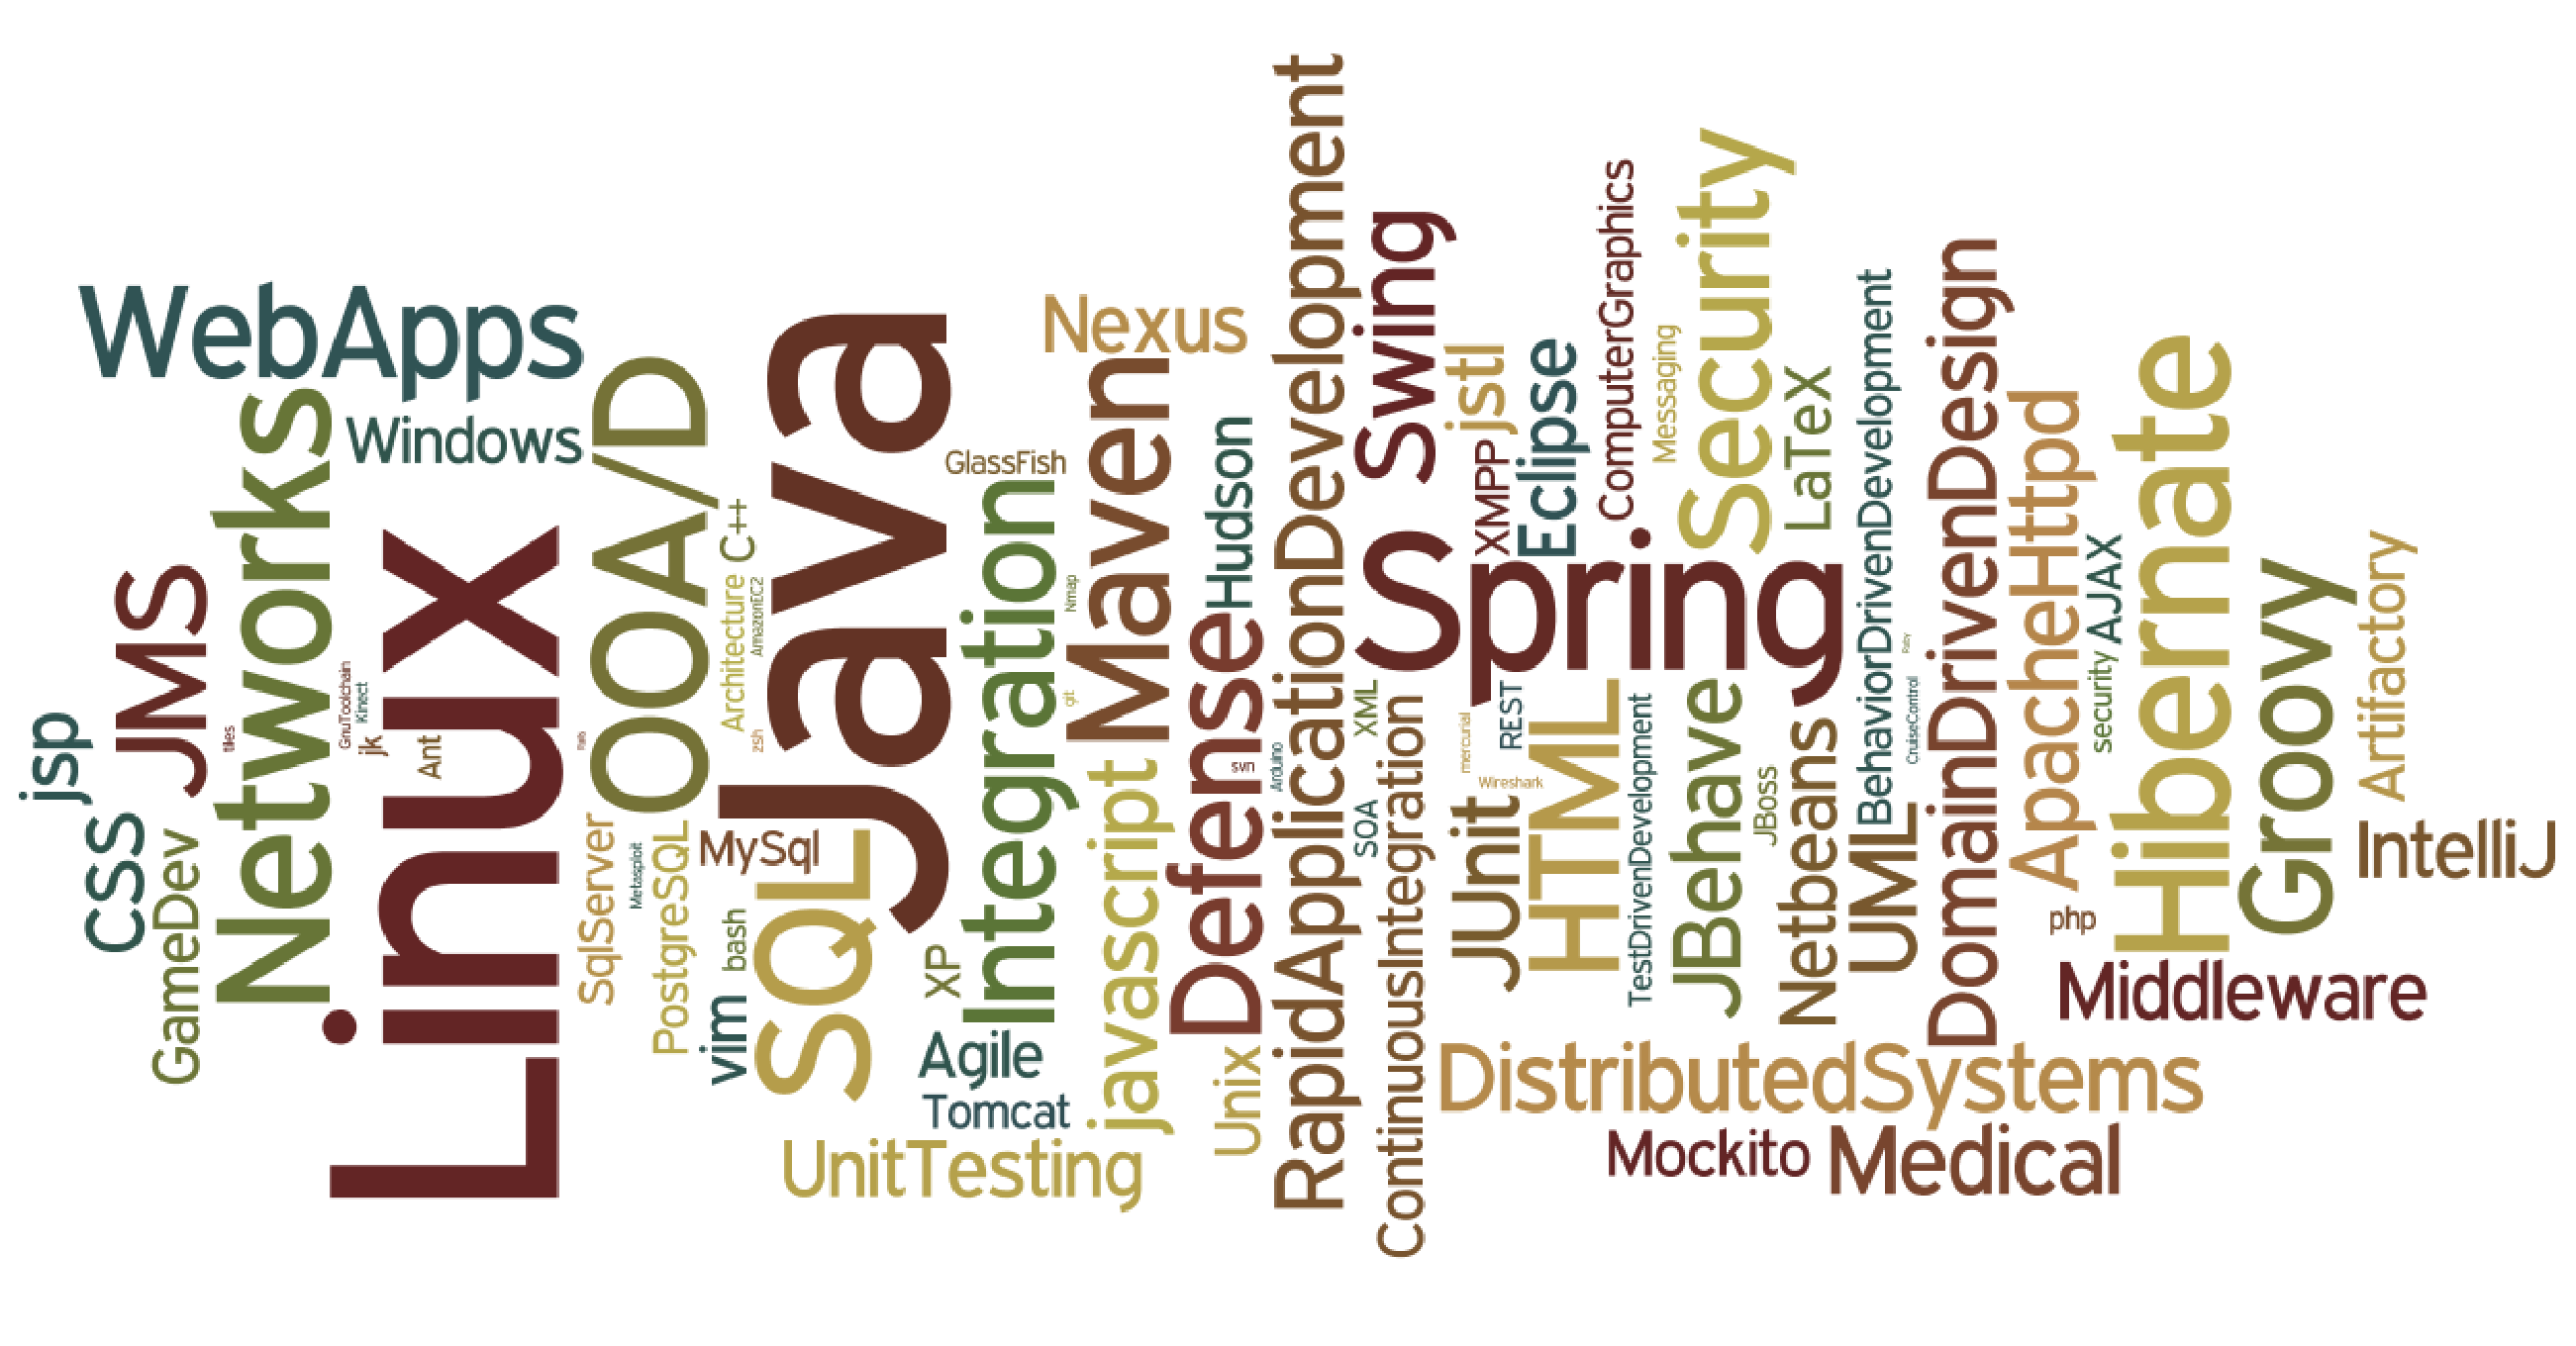
\includegraphics[scale=0.30]{word_cloud3.pdf}

% \begin{figure}[!h]
%   \begin{center}
%     \scalebox{0.35}{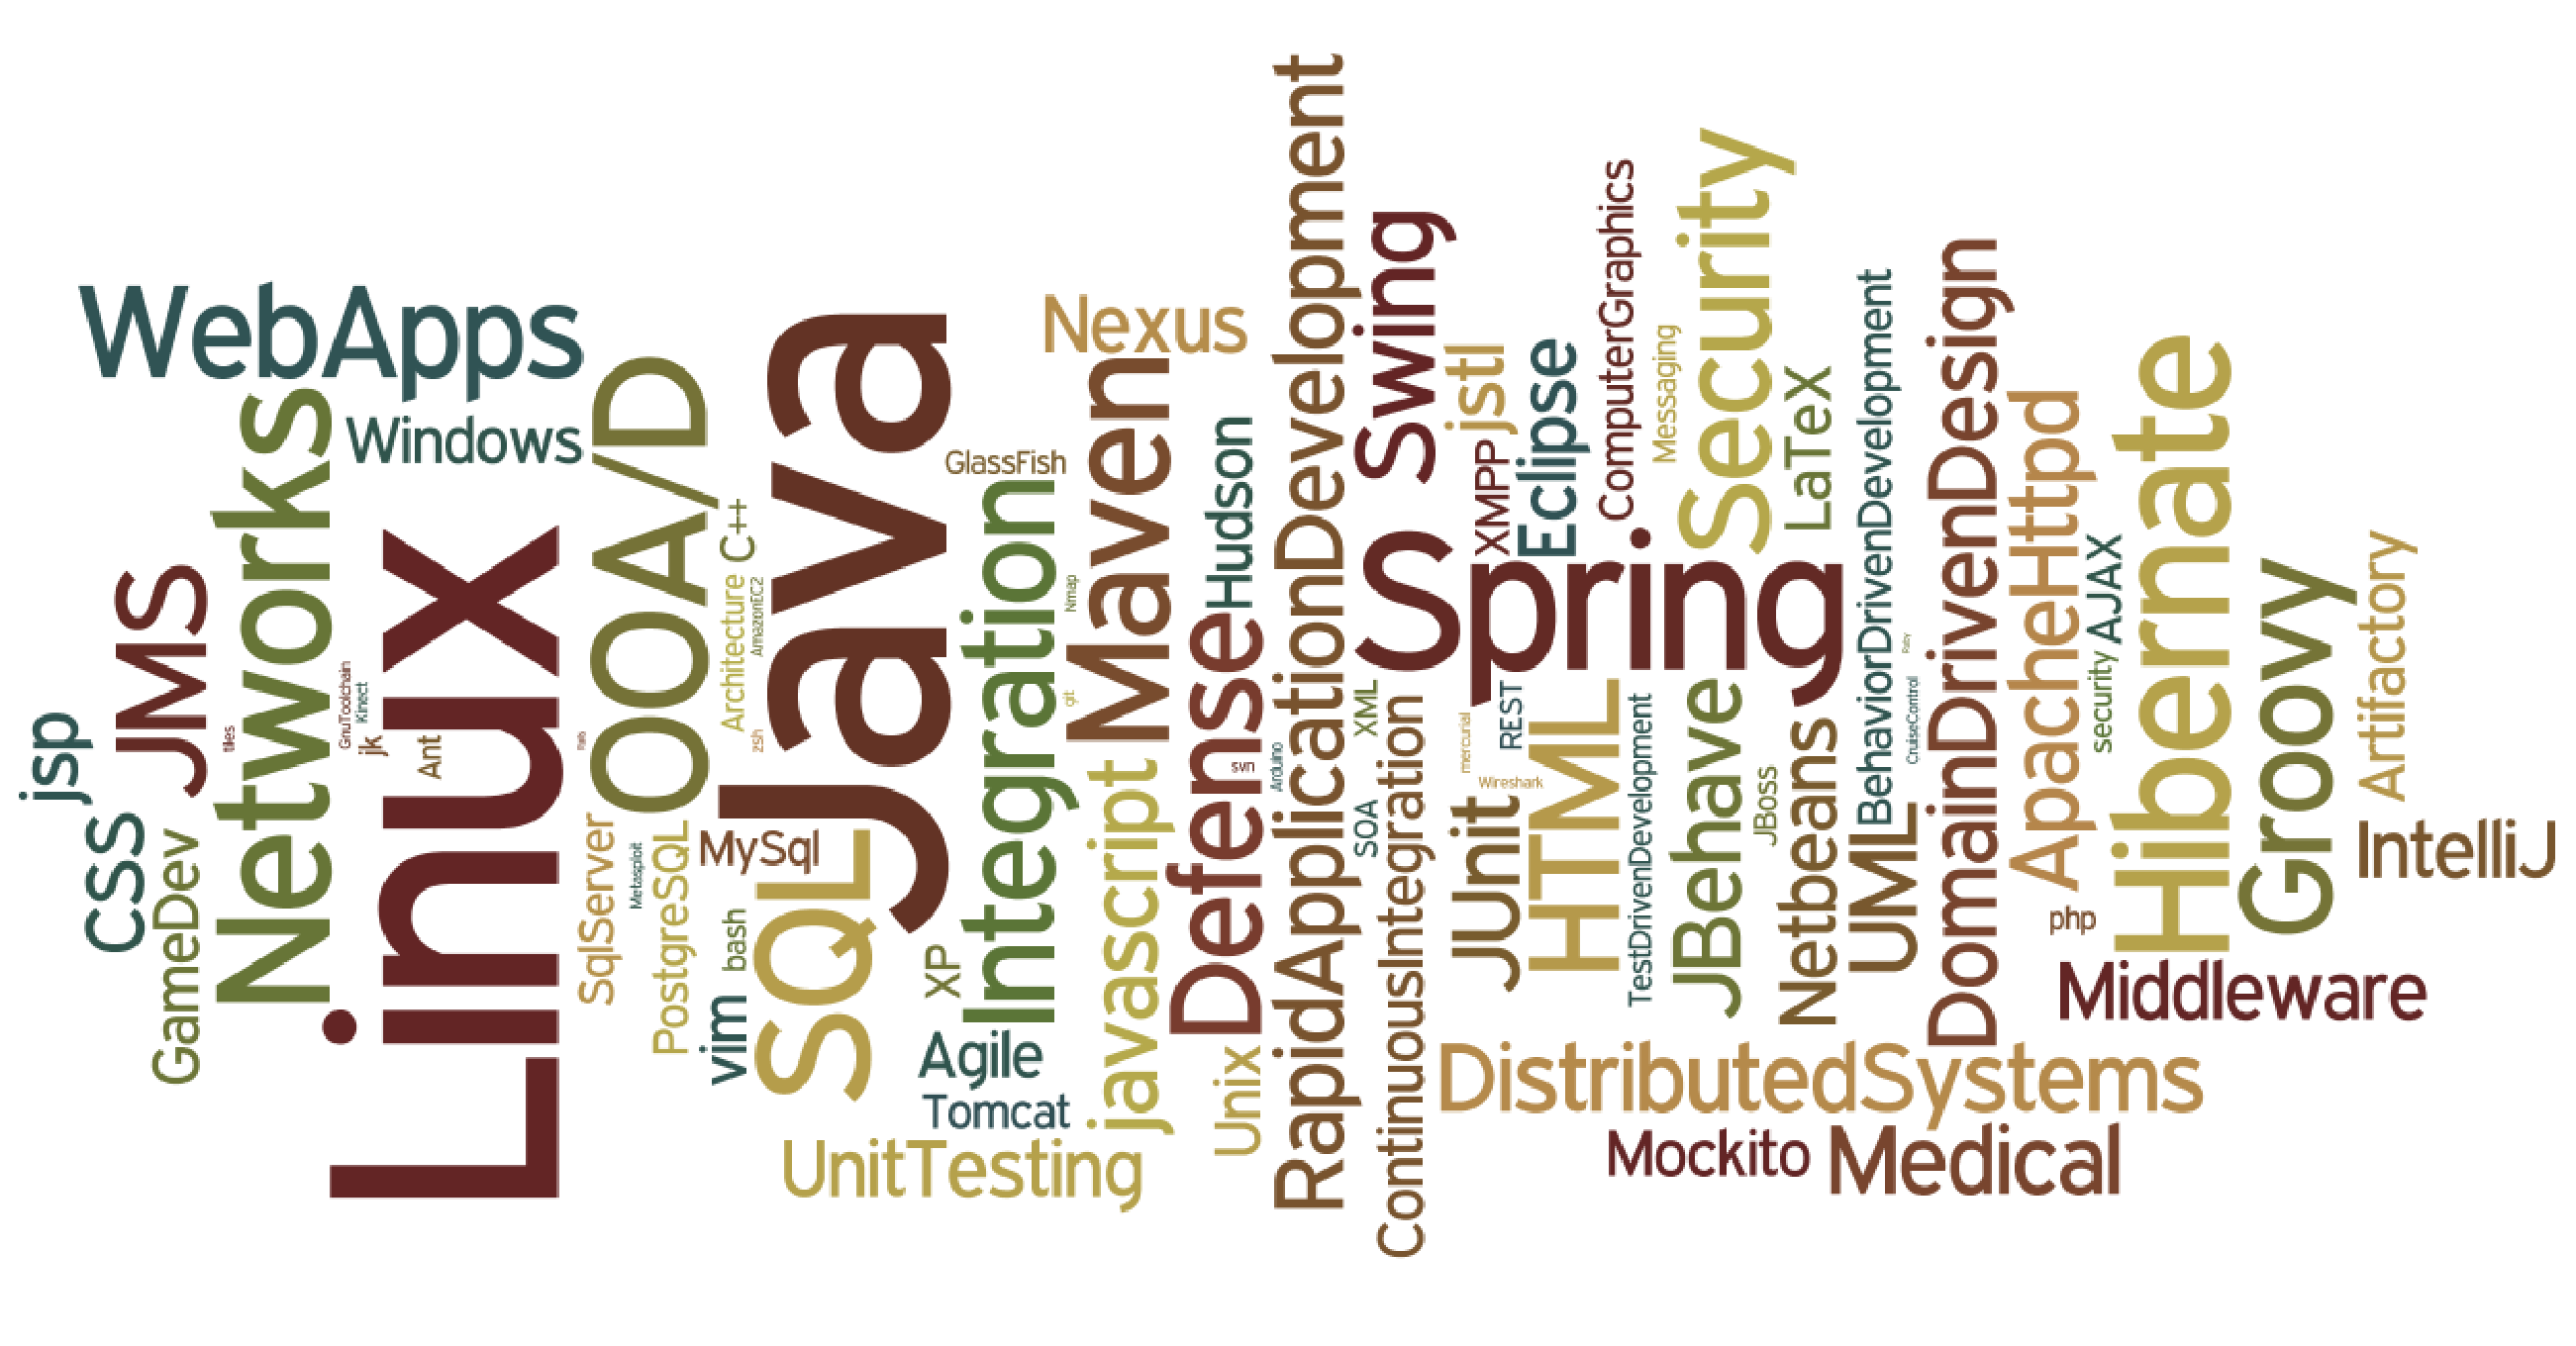
\includegraphics{word_cloud3}}
%   \end{center}
%    \caption{\small A sample}
%    \label{tree}
% \end{figure}



\end{document}

